\documentclass[11pt,letterpaper]{article}
\usepackage[T1]{fontenc}
\usepackage{lmodern,amsmath,amssymb,amsthm,graphicx,booktabs,tabularx,array,xcolor,tikz}
\usepackage[margin=0.96in,top=0.89in,bottom=0.85in,headheight=15pt,headsep=15pt]{geometry}
\usepackage{fancyhdr,enumitem}
\usepackage[colorlinks=true,linkcolor=teal!60!black,urlcolor=teal!65!black,citecolor=teal!60!black,pdftitle={Helly's theorem in intuitionistic primitive recursive arithmetic}]{hyperref}
\definecolor{ink}{HTML}{163A44}
\definecolor{tealproof}{HTML}{006A67}
\definecolor{warm}{HTML}{AD4B26}
\pagestyle{fancy}\fancyhf{}
\fancyhead[L]{\small\sffamily\color{ink} Helly's theorem in iPRA}
\fancyhead[R]{\small\sffamily\color{ink} Constructive geometry}
\fancyfoot[C]{\small\sffamily\thepage}
\setlength{\parindent}{0pt}\setlength{\parskip}{5.4pt plus 0.8pt minus 0.5pt}
\setlist{nosep,leftmargin=*}
\setlength{\emergencystretch}{2em}
\newcommand{\Q}{\mathbb Q}\newcommand{\R}{\mathbb R}\newcommand{\N}{\mathbb N}
\newcommand{\I}{\mathcal I}\newcommand{\Hh}{\mathcal H}
\newcommand{\Hull}{\operatorname{conv}}\newcommand{\eqv}{\simeq}
\newcommand{\Norm}[1]{\lVert #1\rVert_\infty}
\newcommand{\key}[1]{\smallskip\noindent{\sffamily\bfseries\color{ink}#1}\enspace}
\newcommand{\repo}{https://github.com/VladimirReshetnikov/ProveIt}
\newcommand{\pin}{022dfb4c54c22782f927a903f25bcf6491b7eba2}
\newcommand{\basepath}{Logic/PrimitiveRecursiveArithmetic}
\newcommand{\gh}[2]{\href{\repo/blob/\pin/\basepath/#1}{#2}}
\newtheoremstyle{packet}{6pt}{3pt}{\itshape}{}{\sffamily\bfseries\color{tealproof}}{.}{.5em}{}
\theoremstyle{packet}\newtheorem{theorem}{Theorem}\newtheorem{lem}[theorem]{Lemma}
\newtheorem{cor}[theorem]{Corollary}\newtheorem{prop}[theorem]{Proposition}
\renewcommand{\qedsymbol}{\ensuremath{\square}}
\newcommand{\head}[1]{\section{#1}}
\begin{document}
\thispagestyle{plain}
{\color{tealproof}\sffamily\fontsize{10}{12}\selectfont CONSTRUCTIVE GEOMETRY \quad / \quad RESEARCH NOTE}\par
\vspace{0.16in}
{\sffamily\bfseries\color{ink}\fontsize{29}{33}\selectfont Helly's theorem in intuitionistic\\primitive recursive arithmetic\par}
\vspace{0.11in}
{\large A common point, its barycentric certificates, and the boundary for real coordinates}\par
\vspace{0.08in}\textcolor{tealproof}{\rule{\textwidth}{1.1pt}}

For four convex sets in the plane, suppose we know a point in each of the four triple intersections. How can we assemble these four points into a point in all four sets? The two diagonals of a quadrilateral suggest the answer. Where they cross, the same point has two descriptions. Each description avoids two of the given vertices, so one of them avoids any specified vertex. Radon's lemma \cite{radon} supplies such descriptions even when the four points are collinear, repeated, or arranged with one inside the triangle of the others.

\begin{theorem}[Finite rational Helly with certificates]\label{thm:main}
Let $n\ge1$, $d\ge0$, $[n]=\{0,\ldots,n-1\}$, $h=\min(n,d+1)$ and
$\mathcal T=\{T\subseteq[n]: |T|=h\}$. Give one point $p_T\in\Q^d$ for every $T\in\mathcal T$. Uniformly in $n,d$ and this table, primitive recursive functions compute $y\in\Q^d$ and rational numbers $w_{iT}$ satisfying, for every $i<n$,
\begin{equation}
  w_{iT}\ge0,\qquad i\notin T\Rightarrow w_{iT}=0,\qquad
  \sum_T w_{iT}=1,\qquad \sum_T w_{iT}p_T=y.\tag{H}\label{eq:helly}
\end{equation}
iPRA proves these identities and inequalities. Each row can additionally be chosen to have at most $d+1$ nonzero entries.
\end{theorem}

If $p_T$ belongs to every convex set $C_i$ with $i\in T$, row $i$ places $y$ in $C_i$. Thus (H) yields a single exhibited point of the full intersection. For $n\ge d+1$ the hypothesis is precisely a supplied witness for each $(d+1)$-fold intersection. For $n<d+1$ it asks for one point of the entire family. For $n=0$ the origin is a witness and the table of rows is empty.

The rational identities also yield an exact theorem for real polyhedra defined by rational inequalities, where merely asserting local feasibility suffices (p.~\pageref{sec:poly}). For arbitrary regular real inputs they give uniform approximations at every precision (p.~\pageref{sec:real}). Four explicitly presented triangles show that no uniform computable operation can return an exact real point in that generality (p.~\pageref{sec:obstruction}). We also give a fixed-size double-negation formulation. These distinctions matter because in intuitionistic logic an inhabited set carries more information than a set whose emptiness leads to contradiction.

\newpage
\head{The arithmetic statement and convex membership}\label{sec:codes}

We use the first-order theory specified by ProveIt \cite{proveit}. Its variables range over natural numbers. It has the defining equations for all primitive recursive (PR) functions, intuitionistic logic with equality, and induction on quantifier-free formulas. Matrices, lists and graphs below are finite data encoded by numbers. A reference to an arbitrary PR presentation means a schema with that function fixed, or one fixed PR family with numerical parameters.

\key{Codes.} One concrete pairing is $\langle u,v\rangle=(u+v)^2+u$. On a pair, $r=\lfloor\sqrt z\rfloor$ gives $u=z-r^2$ and $v=r-u$. Bounded search computes $r$. Tag the empty list by zero and a cons by $1+\langle u,v\rangle$; fold and lookup with the encoded length or the original code as fuel. Each tail has smaller code. Integers can be signed magnitudes, rationals pairs $(a,b)$ with $b>0$. Equality is $ab'=a'b$ and order uses the same cross products. Addition, multiplication, guarded reciprocal and absolute value are PR. One may reduce by the gcd or work modulo cross equality. Use a fixed default at bad codes, absent indices or zero denominators. Store vectors as length-tagged lists, and subsets of $[n]$ as masks below $2^n$.

\key{A single object-language formula.} Let $\mathsf{Input}(n,d,P)$ check the shapes and positive denominators of a table on $\mathcal T$. For example, use an array indexed by all masks and ignore entries of the wrong cardinality. Let $\mathsf{Check}(n,d,P,Z)$ inspect the output shape, all signs, support and sum tests in (H), coordinate by coordinate. Both return bits. With $H$ the algorithm of Sections~\ref{sec:radon}--\ref{sec:glue}, the universally closed formula is
\[
 \mathsf{Input}(n,d,P)=1\ \longrightarrow\
 \mathsf{Check}(n,d,P,H(n,d,P))=1 .
\]
The sparse version adds a count of each row's strictly positive entries. Bounded conjunction is the test that a bounded sum of failure bits equals zero. Its introduction and elimination follow by quantifier-free induction on the running sum. This device lets every table invariant in the proof be a single bit equality.

\key{From binary convexity to row membership.} Let $M(i,x)$ be an extensional PR membership test. Assume closure under rational binary blends $(1-t)x+tz$ for $0\le t\le1$. Given row $i$, scan its positive terms. The first such term exists by the sum-one test. Set the running point to its input point and its mass to its weight. With current mass $s>0$, adding $w>0$ replaces $x$ by $(s x+w p)/(s+w)$. This is a binary blend with $t=w/(s+w)$, so membership is preserved. The invariant records the mass processed, the cross-multiplied coordinate sums, and the bit $M(i,x)$. At termination $s=1$ and $x=y$. Extensionality handles different codes for the same point. A decidable scan can instead track a separate empty-prefix flag.

More generally (H) supplies a proof for any presentation accepting finite convex-combination certificates, even if membership is rich or witnessed. For externally fixed $n,d$ the local existential statements can be eliminated one by one and all finite convexity arguments unrolled. For variable sizes a witness table, a PR selector, or a suitable witness bound is explicit data. We do not infer a single coded table from an unbounded collection of existentials by a choice principle.

\newpage
\head{Radon's lemma without a rank assumption}\label{sec:radon}

\begin{lem}[Two compatible convex combinations]\label{lem:radon}
From $d+2$ indexed rational points $x_j$ in $\Q^d$ one can compute two nonnegative rational vectors $u,v$, each of mass one, with
$u_j v_j=0$ for every $j$ and $\sum u_jx_j=\sum v_jx_j$.
\end{lem}

Write $x_j=N_j/D_j$ with an integer vector $N_j$ and integer $D_j>0$, using the product of coordinate denominators if needed. Set $s=d+2$ and let $A$ have columns $(D_j,N_j)$. We construct a nonzero integer column $c$ with $Ac=0$. The following elimination, also used by the Lean program, needs no determinant identity.

Start a pool of $s$ columns with $V=I_s$. After processing $t$ rows of $A$, maintain a matrix $V$ of $m$ integer columns, a rational $m\times s$ matrix $L$, and the following invariant:
\[
  m\ge s-t,\qquad A_{<t}V=0,\qquad LV=I_m .
\]
Initially $L=I_s$. For the next row $r$, compute $b_j=r V_j$. If all $b_j$ vanish, retain the pool. Otherwise pick a column $v=V_\ell$ with $a=b_\ell\ne0$. For each $j\ne\ell$ keep the new column and dual row
\[
          V'_j=a V_j-b_jv,\qquad L'_j=L_j/a.
\]
Delete position $\ell$ and relabel in the original order. The new columns annihilate $r$ since $ab_j-b_ja=0$, and they still annihilate every previous row. For $i,j\ne\ell$,
$L'_i V'_j=L_i V_j-(b_j/a)L_iV_\ell=\delta_{ij}$.
The pool loses one column. This proves the invariant by induction on $t$; all entries and matrix assertions are finite rational tests. $L$ can be carried as proof data and omitted from the executable generator.

After $d+1$ rows at least one column $c$ remains. Its dual row has dot product one with it, so a bounded scan finds a nonzero coordinate. Set $z_j=c_j D_j$. The first row of $Ac=0$ gives $\sum z_j=0$ and the other rows give $\sum z_jx_j=0$. Write $z_j^+=\max(z_j,0)$ and $z_j^-=\max(-z_j,0)$. The two sums of parts equal some $M$. If $M=0$, all parts are zero by nonnegativity, contradicting $c\ne0$ and $D_j>0$. Hence $M>0$. Divide the positive and negative parts by $M$ to obtain $u$ and $v$. Their supports are disjoint and the weighted sums agree. This proves Lemma~\ref{lem:radon}, including every deficient-rank case and $d=0$.\hfill$\square$

\key{The independent minor construction in Python.} Apply the same argument's normalization to a kernel relation for the matrix with columns $(x_j,1)$. To find it, enumerate square minors, largest size first. Choose a nonsingular block $B=A_{I,K}$ and a column $j\notin K$. Set $c_j=\det B$, $c_{k_\ell}=-\det(B\text{ with column }\ell\text{ replaced by }A_{I,j})$, all other entries zero. For any row $i$, $(Ac)_i$ is the determinant of $B$ bordered on the right by $A_{I,j}$ and below by $(A_{i,K},A_{ij})$, by expansion along the bottom row. With $i\in I$ it has a repeated row; otherwise it is a larger minor up to sign, hence zero. A row of ones ensures some nonzero minor. Ordinary rational row reduction computes each determinant. Both procedures give the two combinations in the lemma.

\newpage
\head{Gluing the local witnesses}\label{sec:glue}

For every $S\subseteq[n]$ with $|S|\ge h$, build a point $y_S$ and one row $w^S_i$ for each $i\in S$. Require all rows to have mass one and barycentre $y_S$, with positive entries only at $T$ such that $i\in T\subseteq S$. For $|S|=h$, set $y_S=p_S$ and put unit mass on $S$ in each row. These equations initialize the induction.

For $|S|>h$ we have $h=d+1$. Take the first $d+2$ distinct indices $J$ of $S$. For each $j\in J$ the previous level supplies $x_j=y_{S\setminus\{j\}}$. Apply Lemma~\ref{lem:radon} to them and set $y_S=\sum_{j\in J}u_jx_j=\sum_{j\in J}v_jx_j$. To compute row $i$, choose weights $a=v$ if $i\in J$ and $u_i>0$, and choose $a=u$ otherwise. If $i\in J$ then $a_i=0$ in either case. Thus for every $j$ carrying positive $a_j$ the required child row for $i$ exists. Define
\[
 w^S_{iT}=\sum_{\substack{j\in J\\ a_j>0}} a_j w^{S\setminus\{j\}}_{iT}.
\]
All entries are nonnegative. A positive term implies $i\in T\subseteq S\setminus\{j\}$ by the child invariant. Interchange two finite sums to obtain
\[
 \sum_T w^S_{iT}=\sum_j a_j=1,\qquad
 \sum_T w^S_{iT}p_T=\sum_j a_j x_j=y_S .
\]
This proves the next level. At $S=[n]$ it is (H). Distinctions between children throughout are distinctions of indices, so the proof also works when two child points coincide.

\key{Induction audit.} Iterate over $k=h,\ldots,n$. At level $k$ scan masks below $2^n$. The state contains the preceding level and the partially filled next level. A prefix invariant says that every processed eligible mask passes the displayed finite checks; updates read only masks from the completed level. Bounded rational sum rearrangement follows by distributivity and induction on the two prefix lengths with the arrays as parameters. The outer invariant is the single bit testing every eligible row at that level. Both inductions are quantifier-free. List updates, mask scans and every pivot step are PR iterations of fixed transition functions. Nested loops whose bounds are PR in previously computed data remain PR. No bound on rational coefficient size is needed as an extra assumption.

\key{Compressing the proof of membership.} Suppose a final row $w$ has more than $d+1$ positive entries. Take any $d+2$ of them. The construction in Lemma~\ref{lem:radon} gives a nonzero affine dependence $z$ on their points, padded by zeros elsewhere, with entries of both signs. Set
\[
 \theta=\min_{z_T>0}\frac{w_T}{z_T},\qquad w'_T=w_T-\theta z_T.
\]
The minimum exists by a nonempty finite rational scan. All new entries are nonnegative, at least one former positive entry is zero, and no previously absent entry is added. The zero mass and moment of $z$ preserve the row's sum and barycentre. Iterate for at most $|\mathcal T|$ steps, with an idle step once the target size is reached. This proves the sparse conclusion and completes Theorem~\ref{thm:main}.\hfill$\square$

\newpage
\head{Exact feasibility for rational polyhedra}\label{sec:poly}

\begin{theorem}[Helly alternative]\label{thm:poly}
Let each of $C_0,\ldots,C_{n-1}$ be given by a finite list of weak linear inequalities with rational coefficients in $d$ variables. A PR procedure returns either a rational common point or indices of at most $d+1$ sets whose combined system is inconsistent. The same alternative detects feasibility over $\R^d$. In particular, local existential feasibility gives the usual exact Helly conclusion for this presentation without a supplied table of points.
\end{theorem}

The required ingredient is a choice function for each local linear system. Here is the algorithm and its proof. Eliminate the last coordinate $t$, writing a row as $a\cdot x+pt\le b$. Keep each row with $p=0$. A row with $p<0$ gives a lower bound $L(x)=(b-a\cdot x)/p$ and a row with $p>0$ gives an upper bound $U(x)$ by the same formula. For each pair insert $L(x)\le U(x)$ into the projected system. It is a rational weak linear inequality: equivalently multiply the lower row by $p_{\rm upper}>0$ and the upper row by $-p_{\rm lower}>0$, then add.

Every feasible point projects to a feasible point by these implications. Conversely, given a rational point of the projection, choose $t$ as the largest lower bound if any exists. The pairwise inequalities put it below all upper bounds. If there are only upper bounds choose their minimum; if both lists are empty use zero. This gives a rational lift satisfying every old row. In zero dimensions feasibility is exactly the finite test $0\le b$ on the constant rows.

Repeat for $d$ eliminations, retaining the lists to lift in reverse. A level with $m$ rows produces at most $m+m^2$ rows. Both the stack of levels and reconstruction are PR. For a first-order correctness proof, the forward induction fixes a candidate point and checks its coordinate prefixes at successive projected levels. The reverse induction checks the rational prefix just constructed. In each case, the invariant is the bit for a finite list of inequalities. Thus any rational feasible point implies acceptance; acceptance yields a rational feasible output. Real feasibility implies acceptance as well: take the same positive rational linear combinations of true real inequalities down to the zero-dimensional system. One can equivalently carry, with each projected row, its nonnegative rational multipliers on all initial rows. These multipliers start as unit vectors and obey exactly the same scaled additions. Their finite rational invariant shows that rejection exhibits a linear combination with left side zero and right side strictly negative, impossible at any real point.

For $n>0$ scan the $h$-subsets. If a test rejects, output that subset. Otherwise store all selected rational points and apply (H). Each original row is preserved by nonnegative combinations of total weight one, so the resulting point satisfies every group. For $n=0$ return the origin. The alternatives are disjoint by restriction of a feasible point. This proves Theorem~\ref{thm:poly}.\hfill$\square$

The same reasoning covers rational polytopes given by vertices. To test whether the hulls of several finite vertex lists have a common point, introduce a common variable $x$ and one list of nonnegative weights of sum one per hull. Set its weighted vertex sum equal to $x$. Replace each equality by two weak inequalities. Elimination yields a rational local $x$ and witnesses of hull membership. The Helly number is still $d+1$ because the gluing happens in the original $x$-space.

\newpage
\head{A worked example, sharpness, and a centerpoint}

\key{Four triples in the plane.} Let $p_0=(0,0)$, $p_1=(2,0)$, $p_2=(2,2)$ and $p_3=(0,2)$. The point $p_j$ is supplied for the triple omitting $j$, so $C_i$ is known to contain all corners except possibly $p_i$. The two diagonals give
\[
  y=\tfrac12 p_0+\tfrac12 p_2=(1,1)=\tfrac12 p_1+\tfrac12 p_3.
\]
Each $C_i$ contains the two endpoints of at least one of those diagonals. These are precisely the four rows in (H).
\begin{center}
\begin{tabular}{@{}m{0.38\linewidth}m{0.48\linewidth}@{}}
\centering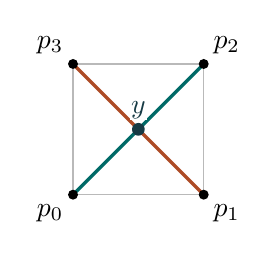
\begin{tikzpicture}[x=0.83cm,y=0.83cm,baseline=(current bounding box.center)]
\draw[gray!55] (0,0) rectangle (2,2);
\draw[tealproof,very thick] (0,0)--(2,2);
\draw[warm,very thick] (2,0)--(0,2);
\foreach \x/\y/\lab/\anch in {0/0/0/north east,2/0/1/north west,2/2/2/south west,0/2/3/south east}
{\fill (\x,\y) circle (1.8pt) node[anchor=\anch] {$p_{\lab}$};}
\fill[ink] (1,1) circle (2.3pt) node[above=3pt,fill=white,inner sep=0.4pt] {$y$};
\end{tikzpicture}
&
\centering\arraybackslash
\begin{tabular}{@{}ll@{}}\toprule
Set & Certificate for $y$\\\midrule
$C_0,\ C_2$ & $\tfrac12(p_1+p_3)$\\[3pt]
$C_1,\ C_3$ & $\tfrac12(p_0+p_2)$\\\bottomrule
\end{tabular}
\end{tabular}
\end{center}

\key{The number $d+1$ is optimal.} For $d\ge1$, take the $d$ halfspaces $x_j\ge0$ and one more, $\sum_j x_j\le-1$. Their full intersection is empty. Omitting the last constraint permits $0$. Omitting constraint $j$ permits $-e_j$. Thus every $d$ members intersect and a smaller local test cannot suffice, even for closed halfspaces with integer coefficients. In dimension zero the single empty set shows that testing no members cannot suffice.

\begin{cor}[Rational centerpoint]\label{cor:cent}
For a nonempty finite multiset of $N$ rational points in $\Q^d$, one can compute a rational point $y$ such that each closed rational halfspace containing $y$ contains at least $\lceil N/(d+1)\rceil$ sample indices.
\end{cor}

Call a subset $S$ of sample indices heavy if $(d+1)|S|>dN$. Form the finite family of hulls of heavy subsets. Any $k\le d+1$ such subsets share a sample index: the sum of their complement sizes is strictly less than $kN/(d+1)\le N$ when $k>0$. Scanning the $N$ indices finds the first survivor. Its sample point supplies a local hull witness. Theorem~\ref{thm:main} yields $y$ in every heavy hull. If a closed rational halfspace containing $y$ held fewer than $N/(d+1)$ points, the points in its open complement would form a heavy subset. Every finite convex combination of those points still satisfies the strict inequality (at least one weight is positive), contradicting $y$'s membership in its hull. All counting, rational comparisons and witnesses in this argument are finite.\hfill$\square$

The centerpoint section of ProveIt's median packet invokes classical finite Helly and then recovers rationality. The preceding argument supplies its rational witness directly, uniformly in the dimension as well as the sample size \cite{median}.

\newpage
\head{Real data at prescribed precision}\label{sec:real}

Use the sup norm. A regular name of a real vector is a rational sequence $u(t)$ satisfying
\[
       \Norm{u(s)-u(t)}\le 2^{-s}+2^{-t} .
\]
Two regular names represent the same vector when their distance tends to zero; equivalently their stage values satisfy the cross bound $\Norm{u(s)-v(t)}\le 2^{-s}+2^{-t}$ for all $s,t$. The equality follows from the triangle inequality and arbitrarily fine rational bounds. A regular name is within $2^{-k}$ of its represented point at stage $k$. Internally this statement means $\Norm{u(t)-u(k)}\le2^{-t}+2^{-k}$ at every stage $t$. Work with a fixed PR family $u(a,T,t)$, where $a$ encodes the numerical input, or with a table of calls at the specified precisions. This formulation uses only the evaluator of the fixed family.

\begin{theorem}[Precision-preserving Helly]\label{thm:approx}
Suppose $u_T$ names a real point in each $C_i$ for $i\in T$. The sets accept finite rational convex combinations of their points and respect equality of names. For any $k$ the construction gives a rational $y_k$ and, for each $i$, a name $v_{i,k}$ in $C_i$ with $\Norm{v_{i,k}-y_k}\le 2^{-k}$. The precision bound is independent of $n$ and $d$.
\end{theorem}

Apply (H) to the rational snapshots $p_T=u_T(k)$, retaining $w_{iT}$. Define the name $v_{i,k}(t)=\sum_Tw_{iT}u_T(t)$. Convexity and the support condition give membership. The regularity bound follows by summing the individual bounds with nonnegative weights of mass one. Moreover,
\[
 \Norm{v_{i,k}(t)-y_k}
 \le\sum_Tw_{iT}\Norm{u_T(t)-u_T(k)}\le 2^{-t}+2^{-k}.
\]
This is the announced first-order precision statement. In particular, $y_k$ belongs to every radius-$2^{-k}$ closed enlargement, in the explicit sense that $v_{i,k}$ is a point of the corresponding set within that distance. Independently computed $y_k$ can vary with $k$, so the regularity of the output sequence would require an additional argument.\hfill$\square$

\key{Interior witnesses yield an exact common point.} Suppose every $u_T$ is supplied with a positive rational $r_T$ whose open sup-norm ball is contained in every $C_i$, $i\in T$. Choose $2^{-k}<\min_T r_T$. For example take $k=D+1$ if $D$ is the largest denominator of these positive fractions. Then the snapshots $u_T(k)$ themselves lie in the required sets, so every row certifies exact membership of the rational $y_k$. This applies to open convex sets with witnessed openness at the specified local points.

\key{Exact closed intervals with real endpoints.} In dimension one, for $n\ge1$ let the sets be $[a_i,b_i]$ with $a_i\le b_i$ and a witness for each pair. Each $a_j\le b_i$ follows from the corresponding witness, or from the individual bound when $i=j$. The point $\max_j a_j$ lies in every interval. One can take the maximum of all rational approximants at the same stage. The inequality $|\max_j u_j-\max_j v_j|\le\max_j|u_j-v_j|$ preserves the regularity bound. In particular, no sign decision on real differences is needed.

\key{From binary to finite real convexity.} For $m\ge1$ nonnegative real weights of sum one, approximate each to error $1/(4m)$. Some rational approximation exceeds $1/(2m)$ since otherwise the weights sum to at most $3/4$. Start with that point and its mass, which is greater than $1/(4m)$. Blend in the other points in order. Each new partial mass is at least the initial one, giving an explicit bound for every division in the binary blend. This proves closure under finite real barycentres at fixed arity without deciding which real weights are zero.

\newpage
\head{Why exact uniform selection fails in the plane}\label{sec:obstruction}

\begin{theorem}[Four triangles]
There is no total computable operation which, from regular names of the vertices of four (possibly degenerate) planar triangles and named points in all four triple intersections, always returns a name of a point in their total intersection. This already fails on a single PR family of inputs with a natural-number parameter.
\end{theorem}

Let $\alpha$ be a binary stream with at most one $1$. Form $a=\sum_{j\;\mathrm{even}}2^{-j-1}\alpha(j)$ and $b=\sum_{j\;\mathrm{odd}}2^{-j-1}\alpha(j)$. Partial sums over $j<t$ have error at most $2^{-t}$. Put
\[
 p_1=(0,0),\quad p_2=(1,0),\quad p_3=(0,a),\quad p_4=(1,-b),
 \qquad C_i=\Hull\{p_j:j\ne i\}.
\]
Each triple omitting $C_i$ contains the explicitly given $p_i$. If an even entry is $1$, then $a>0$ and $b=0$. Hence $C_1=[p_2,p_3]$ and $C_3=[p_1,p_2]$. A common point has the form $(1-t,ta)$ with $ta=0$, so it is $p_2$. In the odd case $a=0$, $b>0$, $C_2=[p_1,p_4]$ and $C_4=[p_1,p_2]$. The corresponding point $(t,-tb)$ on the horizontal segment has $t=0$, so it is $p_1$. For the all-zero stream the whole horizontal segment is common.

\begin{center}
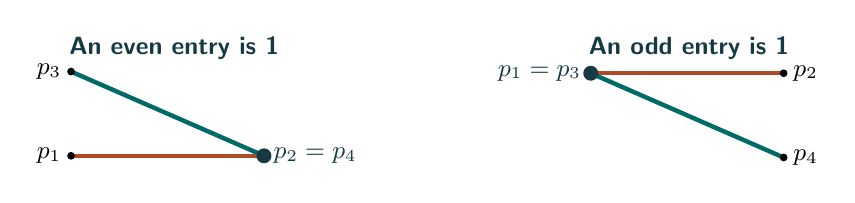
\begin{tikzpicture}[x=2.45cm,y=1.07cm,font=\small]
\begin{scope}
\node[anchor=west,font=\small\sffamily\bfseries,text=ink] at (-0.06,1.28) {An even entry is 1};
\draw[tealproof,line width=1.6pt] (0,1)--(1,0);
\draw[warm,line width=1.6pt] (0,0)--(1,0);
\fill (0,1) circle(1.4pt) node[left] {$p_3$};\fill (0,0) circle(1.4pt) node[left] {$p_1$};
\fill[ink] (1,0) circle(2.7pt) node[right] {$p_2=p_4$};
\end{scope}
\begin{scope}[xshift=6.6cm]
\node[anchor=west,font=\small\sffamily\bfseries,text=ink] at (-0.06,1.28) {An odd entry is 1};
\draw[warm,line width=1.6pt] (0,0.98)--(1,0.98);
\draw[tealproof,line width=1.6pt] (0,0.98)--(1,-0.02);
\fill[ink] (0,0.98) circle(2.7pt) node[left] {$p_1=p_3$};
\fill (1,0.98) circle(1.4pt) node[right] {$p_2$};
\fill (1,-0.02) circle(1.4pt) node[right] {$p_4$};
\end{scope}
\end{tikzpicture}
\end{center}
Each panel shows the two segments that force the common point. A rational approximation $q$ to its first coordinate with error at most $1/8$ suffices to distinguish the forced endpoints: $q\le1/2$ rules out an even $1$ and $q>1/2$ rules out an odd $1$. This yields the lesser limited principle of omniscience (LLPO), which asks for a choice of a parity class free of ones.

\key{A contradiction even for index-based algorithms.} Fix an enumeration of programs. Set $\alpha(e,2s+j)=1$ precisely when program $e$ on input $e$ first halts at step $s$ with output $j\in\{0,1\}$. This is a PR predicate by bounded simulation, and at most one entry is $1$. The input data above are therefore PR in $(e,t)$. A uniform selector would give a total computable bit $F(e)$, equal to 0 when $q\le1/2$ and 1 otherwise. Whenever $e(e)$ halts with a binary output, $F(e)$ differs from that output. Take an index $e$ for the program computing $F$. Its value at $e$ must equal and differ from $F(e)$, a contradiction. This rules out even a selector allowed to inspect the numerical parameter. It leaves the classical existence statement intact.\hfill$\square$

\key{Higher fixed dimensions.} Given such an omission example on $d+2$ vertices in dimension $d$, embed the vertices at height zero in dimension $d+1$ and add one apex at height one. Again take all hulls obtained by omitting a vertex. The hull omitting the apex forces height zero. In every other hull a representation of a height-zero point assigns zero weight to the apex, so the projection belongs to every old hull. Each local witness is still its omitted vertex. Iterating extends the selection obstruction to every fixed $d\ge2$.

\newpage
\head{Double negation and the compact version}

\begin{prop}[Weak exact Helly for fixed finite sizes]\label{prop:weak}
Fix $d,n$ externally and a PR family of regular real local witnesses. There is a fixed PR family of candidate output names and real barycentric rows, indexed by finite branch data $c$, for which iPRA proves $\neg\neg\exists c\,\mathsf{Good}(c)$. Here $\mathsf{Good}$ asserts regularity, nonnegative mass-one rows, the incidence support from (H), and equality of all row barycentres to the candidate. This yields the double negation of a common inhabited intersection for extensional predicates accepting these real barycentres.
\end{prop}

For a regular real $x$ one has $\neg\neg(x<0\lor x=0\lor x>0)$. Indeed, absence of a strict positive or negative certificate gives $-2^{-s}\le x(s)\le2^{-s}$ at every stage, which proves $x=0$. A certificate $x(s)>2^{-s}$ yields a positive rational lower bound $x(s)-2^{-s}$; the negative case is symmetric. One may convert that bound into $2^{-m}$ by a bounded rational computation.

Unroll the pool algorithm of Section~\ref{sec:radon} and the gluing of Section~\ref{sec:glue} at these fixed sizes. With real coordinates use the augmented columns $(1,x_j)$. Branch on the sign of the needed entries and masses. Along any branch with certified outcomes the identical algebra constructs real rows satisfying the mass, support and barycentre equations of (H). For every reciprocal record a positive dyadic lower bound on the absolute denominator. The finite containment and support tests on a branch use its sign information. No compactness step occurs.

Here are the coding details. A fixed finite list of circuit templates suffices: choices are pivot indices, signs, and the side used for each row. The natural code $c$ chooses a template and holds the evidence for strict signs. For names of scalars, $|x(0)|+1$ bounds the represented magnitude. With bounds $M,N$ on the magnitudes, sums at stage $s$ have error at most $2\cdot2^{-s}$, and products of snapshots have error at most $(M+N+1)2^{-s}$ when $s\ge0$. Increase the requested precision by a PR shift large enough for these rational factors. If $|x|\ge\delta=2^{-m}$, evaluate $q=x(t+2m+3)$ and use $1/q$ when $|q|\ge\delta/2$, defaulting to zero otherwise. On a valid branch the guard succeeds and the error is bounded by $2\delta^{-2}2^{-t-2m-3}<2^{-t}$. These rules compose into fixed PR functions of input, $c$ and precision, total also on malformed branches. Their stagewise estimates justify equality and order in the finite field calculations. The row predicates in $\mathsf{Good}$ can be written entirely as rational bounds at all stages.

To combine tests, use $\neg\neg A$ and $A\to\neg\neg B$ to infer $\neg\neg B$: under $\neg B$, the second premise gives $\neg A$, contradicting the first. Apply this rule successively to each sign decision with its strict witness packaged existentially. Because $d,n$ are external numerals, the construction has finite fixed depth; this is a metatheoretic iteration of intuitionistic proofs. The result supplies no choice of branch. This proves Proposition~\ref{prop:weak}.\hfill$\square$

\key{Countably many compact sets.} The classical infinite version uses the finite intersection property in a compact set \cite{target}. For a stream $\alpha$ as above, let $I_t=[0,1]$ until a $1$ occurs before stage $t$, and thereafter $I_t=\{1\}$ after an even event or $I_t=\{0\}$ after an odd event. These are nested rational compact intervals. Every nonempty finite subfamily has a rational witness from its latest interval. Any common real selects a parity just as on p.~\pageref{sec:obstruction}. With the same bounded simulation, uniform exact selection fails already on this line example.

There is a positive modulus version. Let PR rational witnesses $x_t$ belong to the first $t+1$ closed sets. Suppose their intersection at stage $m(k)$ has diameter at most $2^{-k}$, for a given PR $m$. Put $M(k)=\max(k,m(0),\ldots,m(k))$. For $j\ge k$ both $x_{M(j)}$ and $x_{M(k)}$ lie in the first $m(k)+1$ sets. Their distance is at most $2^{-k}$. Thus $k\mapsto x_{M(k)}$ is a regular name, eventually witnessed in each fixed set. Sequential closedness for the given name presentation puts its limit in every set.

\newpage
\head{Lean verification and the object-theory endpoint}\label{sec:lean}

\key{The checked geometric theorem.} The companion \texttt{lean/Helly.lean} develops the rational finite theorem in Lean 4 with \texttt{Std} as its only import. It defines its own rational points and convexity. The declaration \texttt{ConstructiveHelly.QPoint.hellyExact} returns a point with proofs of membership in every member of a finite indexed family. Its only local geometric input consists of witnesses for the duplicate-free lists of $h=\min(n,d+1)$ labels. The Radon operation is implemented and proved total in every dimension.

\begin{center}\begin{tabularx}{\linewidth}{@{}p{.31\linewidth}X@{}}\toprule
\textbf{Lean definitions} & \textbf{Mathematical content}\\\midrule
\texttt{QPoint}, \texttt{equiv}, \texttt{blend} & Integer vector and positive common denominator, cross equality coordinatewise, and a rational convex blend with strictly positive integer weights. Endpoints of a segment need no blend.\\[3pt]
\texttt{ConvexSet}, \texttt{HullTree} & An extensional predicate closed under blends. An indexed binary tree whose leaves are points and whose nodes store the two positive weights minus one.\\[3pt]
\texttt{RadonCertificate}, \texttt{avoid} & Two trees with disjoint leaf supports and equal values. Given one exceptional position, the common value belongs to a convex set containing every other point.\\[3pt]
\texttt{kernelPool}, \texttt{radon\_complete} & The integer pool computes an affine dependence. Lean proves a nonempty pool, all annihilation equations, a nonzero survivor, and agreement of the trees formed from its signed masses.\\[3pt]
\texttt{solve}, \texttt{QPoint.helly} & Recursion on the size of the family. Each chosen deletion produces a child witness. The proved Radon operation and \texttt{avoid} produce the common point.\\\bottomrule
\end{tabularx}\end{center}

The proof of nonzeroness in Lean uses an alternative to the dual matrix. Initially each unit column has a private coordinate, where it is nonzero and all other columns vanish. When the pivot column is removed, on the private coordinate of any surviving $w$ the new column equals $a w$ since the pivot vanishes there. Every other surviving column remains zero there. Thus the private-coordinate property persists and each survivor is nonzero. This also admits a finite bit test in iPRA.

The general interface \texttt{QPoint.helly} takes local data on lists of at most $d+1$ positions. For an $h$-subset table, remove repeated labels from a small query, then add unused labels until its support has size $h$. Its table entry witnesses the original query. This is the conversion used by the finite-family endpoint; lookup in an unordered table can sort the labels first. Deletion recursion is the tree evaluation of the subset computation on p.~\pageref{sec:glue}.

\key{Further checked results.} The file \texttt{lean/Precision.lean} verifies the two-sided weighted error estimate for regular names and snapshots, coordinatewise after clearing denominators. The file \texttt{lean/SelectionBoundary.lean} proves common rational witnesses for every finite prefix in the interval example. It also proves that a single rational approximation within $1/8$ of every interval excludes a parity, and derives the diagonal contradiction given an index for the selector. The bounded machine simulation and the triangle reduction are supplied in the mathematical argument. The exact-arithmetic Python program builds the flattened rows (H), checks them independently of the construction, and optionally makes each row sparse. The checked Lean geometric theorem uses hull trees and membership proofs. Lean 4.19.0 reports only \texttt{propext} and \texttt{Quot.sound} as axioms of \texttt{QPoint.hellyExact}.

\newpage
\head{Compiling the arithmetic proof in ProveIt}

The checked Lean geometry is a metatheoretic theorem. ProveIt's object-language endpoint has type \( (\texttt{[]} : \texttt{List (Fm PTm 0)})\;\vdash_{\texttt{PRAAx}}\;\varphi \), with $\varphi$ the universal closure from p.~\pageref{sec:codes}. The following gives a route to that separate formalization using the pinned tree \cite{proveit}.

\begin{enumerate}[leftmargin=1.8em,itemsep=4pt]
\item \textbf{Code the finite data.} Build the tuple, mask and array terms with \gh{Derivations/Lean/IPRADerivations/Core/Pairing.lean}{\texttt{Core/Pairing}}. Fix decoding defaults and give each parser a PR well-formedness bit. Derive entry-after-update by induction on the list index. Use the fixed-arity PR symbol constructors in \texttt{Core/Definitions} to compile loops into primitive recursion on an explicit bound with one coded state.
\item \textbf{Reflect arithmetic checks.} Use \gh{Derivations/Lean/IPRADerivations/Analysis/RationalArithmetic.lean}{\texttt{Analysis/RationalArithmetic}} for normalized operations and cross equality. Construct the guarded reciprocal by swapping absolute numerator and denominator and restoring the sign. Prove its product equation under nonzero input by cross multiplication. Use \gh{Derivations/Lean/IPRADerivations/Analysis/RationalFiniteSum.lean}{\texttt{Analysis/RationalFiniteSum}} for row masses and coordinates, and \gh{Derivations/Lean/IPRADerivations/Core/BoundedSums.lean}{\texttt{Core/BoundedSums}} to reflect every nested finite check. The scan returning the first successful index records either a valid hit or failure of every input examined so far.
\item \textbf{Prove an object-level Radon constructor.} The inner induction checks the row elimination identities coordinatewise. For each matrix state take a single bit verifying pool length, prior row annihilation, and either the dual matrix identities or the private-coordinate marks. In the latter case retain the surviving marks by deleting the pivot's mark along with the pivot. The outer induction uses \gh{Derivations/Lean/IPRADerivations/Core/Basic.lean}{\texttt{Core/Basic.ind}} on the processed row count. Prove positive and negative masses agree and cannot be zero. Normalize using the guarded reciprocal. This route handles a dimension supplied as input. The existing \gh{Derivations/Lean/IPRADerivations/Algebra/DeterminantLaws.lean}{\texttt{Algebra/DeterminantLaws}} supplies determinant laws for each externally fixed matrix size.
\item \textbf{Prove the dynamic-program invariant.} Define explicit terms for level initialization, child mask lookup, the sign test selecting a side, and accumulation of the parent row. Reflect the prefix bit of Section~\ref{sec:glue}. Its preservation follows from disjointness, the mass-one tests and the moment identities. Close the $[n]$ mask by universal introduction. For sparsity add the support count and the invariant that each non-idle step strictly reduces it. Applying the theorem to a specific PR membership predicate uses the running blend invariant on p.~\pageref{sec:codes}.
\end{enumerate}
These steps specify the remaining object-logic work. The archive includes the human proof and kernel-checked Lean geometry. The uniform certificate formula still awaits a serialized \texttt{Prf PRAAx} derivation.

\begin{thebibliography}{9}\small
\bibitem{target} \href{https://en.wikipedia.org/wiki/Helly\%27s_theorem}{Helly's theorem}. Target statement, finite and infinite formulations.
\bibitem{radon} J. Radon, \href{https://doi.org/10.1007/BF01464231}{Mengen konvexer K\"orper, die einen gemeinsamen Punkt enthalten}. \emph{Math. Ann.} 83 (1921), 113--115. E. Helly, \emph{\"Uber Mengen konvexer K\"orper mit gemeinschaftlichen Punkten}. \emph{Jahresber. DMV} 32 (1923), 175--176.
\bibitem{proveit} V. Reshetnikov, \gh{README.md}{ProveIt, Primitive recursive arithmetic} and \gh{Derivations/README.md}{Derivations}. Repository snapshot \texttt{022dfb4c54c2}.
\bibitem{median} ProveIt, \gh{docs/proofs/probability/median_ipra_constructive_proofs/paper/median_ipra.tex}{Median iPRA packet}, subsection \emph{Centerpoints}, same snapshot.
\end{thebibliography}
\end{document}
